\documentclass{standalone}

\usepackage{pgfplots}
\pgfplotsset{compat=newest}

\begin{document}
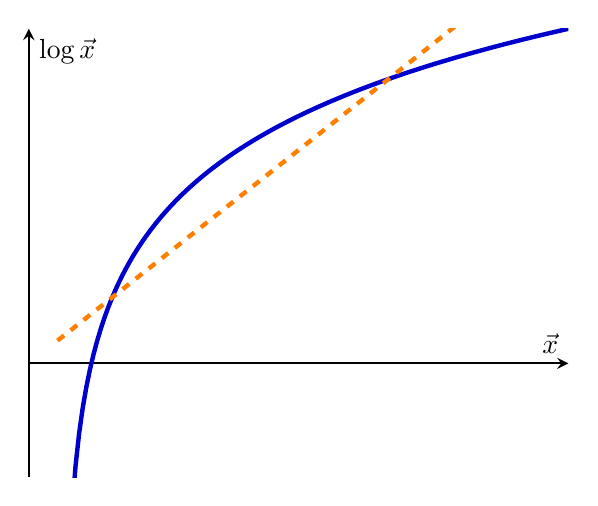
\begin{tikzpicture}
  \begin{axis}[
      axis lines=middle,
      xtick=\empty,
      ytick=\empty,
      ylabel=$\log\vec x$,
      xlabel=$\vec x$,
      xmin=0,
      ymin=-1,
      thick,
      decoration={name=none},
    ]
    \addplot[no marks,blue!80!black,ultra thick,samples=150,domain=1:150] {ln(x-10)-2};
    \draw[orange,dashed,ultra thick] (axis cs:8, 0.2) -- (axis cs:120, 3);
  \end{axis}
\end{tikzpicture}
\end{document}
